%-------------------------------------------------------------------------------
%                      Template Naskah Skripsi
%               	Berdasarkan format JTETI FT UGM
% 						(c) @gunturdputra 2014
%-------------------------------------------------------------------------------

%Template pembuatan naskah skripsi.
\documentclass{jtetiskripsi}

%Untuk prefiks pada daftar gambar dan tabel
\usepackage[titles]{tocloft}
\renewcommand\cftfigpresnum{Gambar\  }
\renewcommand\cfttabpresnum{Tabel\   }

%Untuk hyperlink dan table of content
\usepackage{hyperref}
\newlength{\mylenf}
\settowidth{\mylenf}{\cftfigpresnum}
\setlength{\cftfignumwidth}{\dimexpr\mylenf+2em}
\setlength{\cfttabnumwidth}{\dimexpr\mylenf+2em}

%Untuk Bold Face pada Keterangan Gambar
\usepackage[labelfont=bf]{caption}

%Untuk caption dan subcaption
\usepackage{caption}
\usepackage{subcaption}


%-----------------------------------------------------------------
%Disini awal masukan untuk data proposal skripsi
%-----------------------------------------------------------------
\titleind{PENGEMBANGAN SISTEM MONITORING SISTEM MICROSERVICES UNTUK MENINGKATKAN OBSERVABILITY}

\fullname{HARITS RIZKAL ALIAMDY}

\idnum{19/439814/TK/48544}

\approvaldate{3 Februari 2014}

\degree{Sarjana Teknik Elektro}

\yearsubmit{2023}

\program{Teknologi Informasi}

\dept{Teknik Elektro dan Teknologi Informasi}

\firstsupervisor{Ir. Sujoko Sumaryono, M.T}
\firstnip{196104181988031001}

\secondsupervisor{Bimo Sunarfri Hantono, S.T., M.Eng.}
\secondnip{1977 0131 2002 12 1 003}

%-----------------------------------------------------------------
%Disini akhir masukan untuk data proposal skripsi
%-----------------------------------------------------------------

\begin{document}

\cover

\approvalpage

%-----------------------------------------------------------------
%Disini awal masukan Acknowledment
%-----------------------------------------------------------------
\acknowledgment
\begin{flushright}
\emph{Untuk Ibu, Bapak,\\dan Adik-adikku tercinta.}
\end{flushright}

%-----------------------------------------------------------------
%Disini awal masukan untuk Prakata
%-----------------------------------------------------------------
\preface
Assalamu'alaikum Wr. Wb.

\vspace{0.5cm}

Puji syukur penulis panjatkan ke hadirat Allah SWT karena hanya dengan rahmat dan hidayah-Nya, Tugas Akhir ini dapat terselesaikan tanpa halangan berarti. Keberhasilan dalam menyusun laporan Tugas Akhir ini tidak lepas dari bantuan berbagai pihak yang mana dengan tulus dan ikhlas memberikan masukan guna sempurnanya Tugas Akhir ini. Oleh karena itu dalam kesempatan ini, dengan kerendahan hati penulis mengucapkan terima kasih kepada:

\begin{enumerate}
\item{Bapak Sarjiya, S.T., M.T., Ph.D., selaku Ketua Jurusan Teknik Elektro dan Teknologi Informasi Fakultas Teknik Universitas Gadjah Mada,}
\item{Bapak Sigit Basuki Wibowo, S.T., M.Eng. selaku dosen pembimbing pertama yang telah memberikan banyak bantuan, bimbingan, serta arahan dalam Tugas Akhir ini,}
\item{Bapak Bimo Sunarfri Hantono, S.T., M.Eng. selaku dosen pembimbing kedua yang juga telah memberikan banyak bantuan, bimbingan, serta arahan dalam Tugas Akhir dan kegiatan-kegiatan yang lain,}
\item{Bapak Warsun Najib, S.T., M.Sc. selaku dosen pembimbing akademis penulis dan juga dosen pembimbing lapangan penulis pada KKN-PPM UGM 2013 Unit SLM07,}
\item{Seluruh Dosen di Jurusan Teknik Elektro dan Teknologi Informasi FT UGM, yang tidak bisa disebutkan satu-satu, atas ilmu dan bimbingannya selama penulis berkuliah di JTETI,}
\item{Ibu dan Bapak yang selama ini telah sabar membimbing, mengarahkan, dan mendoakan penulis tanpa kenal lelah untuk selama-lamanya, dan}
\item{Cantumkan pihak-pihak lain yang ingin anda berikan ucapan terimakasih.}
\end{enumerate}

Penulis menyadari bahwa penyusunan Tugas Akhir ini jauh dari sempurna. Kritik dan saran dapat ditujukan langsung pada e-mail atau \emph{mention} langsung pada akun \emph{twitter} saya. Akhir kata penulis mohon maaf yang sebesar-besarnya apabila ada kekeliruan di dalam penulisan Tugas Akhir ini.

\vspace{0.5cm}

Wassalamu'alaikum Wr. Wb.

\begin{tabular}{p{7.5cm}c}
&Yogyakarta, 15 Januari 2014\\
&\\
&\\
&\textbf{Penulis}
\end{tabular}

%-----------------------------------------------------------------
%Disini akhir masukan untuk muka skripsi
%-----------------------------------------------------------------
\tableofcontents
\addcontentsline{toc}{chapter}{DAFTAR ISI}
\listoftables
\addcontentsline{toc}{chapter}{DAFTAR TABEL}
\listoffigures
\addcontentsline{toc}{chapter}{DAFTAR GAMBAR}

%-----------------------------------------------------------------
%Daftar Singkatan [Optional]
%-----------------------------------------------------------------
\singkatan
\noindent

\begin{tabular}{p{20pt}p{3pt}l}
\textbf{A}\\
AJAX & & Asynchronous JavaScript and XML\\
AP & & Access Point\\
API & & Application Programming Interface\\
\\
\end{tabular}

\begin{tabular}{p{20pt}p{3pt}l}
\textbf{C}\\
CLI & & Command Line Interface\\
\\
\end{tabular}

\begin{tabular}{p{20pt}p{3pt}l}
\textbf{C}\\
DFM & & Discovered Full Mesh\\
\\
\end{tabular}

\begin{tabular}{p{20pt}p{3pt}l}
\textbf{E}\\
ERD & & Entity Relationship Diagram\\
\\
\end{tabular}

\begin{tabular}{p{20pt}p{3pt}l}
\textbf{F}\\
FTDI & & Future Technology Devices International\\
FUSE & & Filesystem in Userspace\\
\\
\end{tabular}

\begin{tabular}{p{20pt}p{3pt}l}
\textbf{I}\\
IP & & Internet Protocol\\
\\
\end{tabular}

\begin{tabular}{p{20pt}p{3pt}l}
\textbf{J}\\
JTETI & & Jurusan Teknik Elektro dan Teknologi Informasi\\
\\
\end{tabular}

\begin{tabular}{p{20pt}p{3pt}l}
\textbf{L}\\
LAN & & Local Area Network\\
\\
\end{tabular}

\begin{tabular}{p{20pt}p{3pt}l}
\textbf{O}\\
OSI & & Open Systems Interconnection\\
\\
\end{tabular}

\begin{tabular}{p{20pt}p{3pt}l}
\textbf{R}\\
RF & & Radio Frequency\\
\\
\end{tabular}

\begin{tabular}{p{20pt}p{3pt}l}
\textbf{S}\\
SDLC & & Software Development Life Cycle\\
SFTP & & Secure Shell File Transfer Protocol\\
SSHFS & & Secure Shell Filesystem\\
\\
\end{tabular}

\begin{tabular}{p{20pt}p{3pt}l}
\textbf{U}\\
UGM & & Universitas Gadjah Mada\\
USB & & Universal Serial Bus\\
\\
\end{tabular}

\begin{tabular}{p{20pt}p{3pt}l}
\textbf{V}\\
VRS & & Virtual Routing Structure\\
\\
\end{tabular}

\begin{tabular}{p{20pt}p{3pt}l}
\textbf{W}\\
WAP & & Wireless Access Point\\
WIT & & Western Indonesian Time\\
WLAN & & Wireless Local Area Network\\
WSN & & Wireless Sensor Network\\
\end{tabular}

%-----------------------------------------------------------------
%Disini awal masukan Intisari
%-----------------------------------------------------------------
\begin{abstractind}
Lorem ipsum dolor sit amet, consectetur adipisicing elit, sed do eiusmod tempor incididunt ut labore et dolore magna aliqua. Ut enim ad minim veniam, quis nostrud exercitation ullamco laboris nisi ut aliquip ex ea commodo consequat. Duis aute irure dolor in reprehenderit in voluptate velit esse cillum dolore eu fugiat nulla pariatur. Excepteur sint occaecat cupidatat non proident, sunt in culpa qui officia deserunt mollit anim id est laborum.

Sed ut perspiciatis unde omnis iste natus error sit voluptatem accusantium doloremque laudantium, totam rem aperiam, eaque ipsa quae ab illo inventore veritatis et quasi architecto beatae vitae dicta sunt explicabo. Nemo enim ipsam voluptatem quia voluptas sit aspernatur aut odit aut fugit, sed quia consequuntur magni dolores eos qui ratione voluptatem sequi nesciunt.


\bigskip
\noindent
\textbf{Kata kunci :} \emph{wireless sensor network}, \emph{Internet Protocol}, WiFi, interoperabilitas.
\end{abstractind}

\begin{abstracteng}
\emph{
Lorem ipsum dolor sit amet, consectetur adipisicing elit, sed do eiusmod tempor incididunt ut labore et dolore magna aliqua. Ut enim ad minim veniam, quis nostrud exercitation ullamco laboris nisi ut aliquip ex ea commodo consequat. Duis aute irure dolor in reprehenderit in voluptate velit esse cillum dolore eu fugiat nulla pariatur. Excepteur sint occaecat cupidatat non proident, sunt in culpa qui officia deserunt mollit anim id est laborum.}

\emph{Sed ut perspiciatis unde omnis iste natus error sit voluptatem accusantium doloremque laudantium, totam rem aperiam, eaque ipsa quae ab illo inventore veritatis et quasi architecto beatae vitae dicta sunt explicabo. Nemo enim ipsam voluptatem quia voluptas sit aspernatur aut odit aut fugit, sed quia consequuntur magni dolores eos qui ratione voluptatem sequi nesciunt.}

\bigskip
\noindent
\textbf{\emph{Keywords :}} \emph{wireless sensor network, Internet Protokol, WiFi, interoperability}.
\end{abstracteng}
%-----------------------------------------------------------------
%Disini akhir masukan Intisari
%-----------------------------------------------------------------

%-----------------------------------------------------------------
%Disini awal masukan untuk Bab
%-----------------------------------------------------------------
%!TEX root = ./template-skripsi.tex
%-------------------------------------------------------------------------------
% 								BAB I
% 							LATAR BELAKANG
%-------------------------------------------------------------------------------

\chapter{LATAR BELAKANG}

\section{Latar Belakang Masalah}
Saat ini, perkembangan teknologi sangatlah cepat, terlebih dengan adanya revolusi industri 4.0. Dengan perkembangan yang cepat itu kebutuhan akan perangkat lunak pun semakin banyak dan semakin kompleks. Menurut State of the Developer Nation report pada edisi 20 terdapat 24.3 juta pengembang perangkat lunak di seluruh dunia yang akan meningkat 20\% setiap tahunnya dan diperkirakan pada tahun 2030 akan ada 45 juta pengembang perangkat lunak\cite{DeveloperReport}. Hal tersebut menggambarkan betapa tingginya demand untuk pembuatan perangkat lunak. Perkembangan seperti ini membuat beberapa konsep dan cara pengembangan perangkat lunak yang sebelumnya dipakai menjadi tidak relevan karena kebutuhan perangkat lunak yang semakin banyak dan kompleks. Salah satunya adalah arsitektur monolith pada perangkat lunak, dimana sebuah perangkat lunak dibangun sebagai satu kesatuan utuh. Pada arsitektur monolith tiap bagian perangkat lunak terikat dengan erat (\emph{tightly coupled}) sehingga ketika aplikasi sudah begitu besar akan sangat sulit untuk melakukan perubahan karena ada kemungkinan perubahan tersebut berdampak pada bagian lain di perangkat lunak. Hal ini berdampak pada waktu pengembangan yang lebih lambat, karena para pengembang harus menguji dan \emph{deploy} seluruh aplikasi setiap kali terjadi perubahan.

Permasalahan yang umum terjadi pada arsitektur monolith coba diselesaikan oleh arsitektur microservices. Microservices merupakan salah satu jenis arsitektur perangkat lunak yang sedang populer belakangan ini. microservices membagi perangkat lunak menjadi beberapa bagian yang lebih kecil yang disebut servis. Masing-masing servis berjalan secara terpisah independen berdasarkan domain bisnisnya. Arsitektur microservices hadir untuk menyelesaikan masalah atau limitasi pada arsitektur tradisional monolith yang diantaranya kemudahan dalam proses-proses maintainability, reusability, scalability, availability, dan automated deployment.

Meskipun arsitektur miroservices menyelesaikan banyak permasalahan yang ada pada arsitektur monolith, terdapat masalah dan tantangan baru pada bagian monitoring dan memahami keseluruhan sistem secara utuh. Dikarenakan jumlah servis yang banyak dan tiap servis terdistribusi secara independen, cukup sulit untuk melacak aliran data dan mengetahui bagian yang bermasalah atau menjadi \emph{bottle-neck} pada sistem. Karena hal tersebutlah observability ada.

Secara sederhana observability merujuk pada kemampuan untuk mengetahui apa yang terjadi (\emph{internal state}) pada sebuah sistem, tidak peduli betapa simpel atau kompleksnya sistem tersebut berdasarkan keluaran yang dihasilkan. dengan kata lain, observability memungkinkan pengembang untuk mengetahui dan menganalisa perilaku dan keadaan dari sistem yang terdistribusi melalui berbagai macam data telemetri yang dikumpulkan.Dengan menerapkan observability pada sebuah sistem microservices yang terdistribusi, para pengembang dapat mengetahui bagaimana antar service berkomunikasi dan berinteraksi sehingga dapat mengatasi masalah yang terjadi atau yang mungkin terjadi pada sistem. Sebagai contoh, pengembang dapat dengan mudah mengidentifikasi bagian mana yang lambat pada sistem sehingga dapat segera dioptimalkan.

Pada penulisan skripsi kali ini, penulis akan mengembangkan suatu sistem penerapan observability pada sebuah sistem microservices berdasar pada 3 pilar observability yaitu metrics, traces, dan logs.

\section{Rumusan Masalah}
Berdasarkan latar belakang yang telah dituliskan sebelumnya, terdapat masalah dan tantangan dalam upaya mengetahui keadaan internal suatu sistem perangkat lunak berbasis microservices. Masalah tersebut muncul karena arsitektur microservices membagi sistem menjadi bagian-bagian yang lebih kecil yang secara alamiah akan membuat sistem perangkat lunak menjadi lebih kompleks. Permasalahan yang muncul pada arsitektur microservices terkait upaya mengetahui keadaan internal sistem terebut diantaranya adalah:
\begin{enumerate}
\item Bagaimana cara untuk mengembangkan tools monitoring yang dapat meningkatkan observability pada sistem microservices?
\item Bagaimana cara mengumpulkan data telemetri dari masing-masing servis yang terdistribusi secara independen dan memiliki teknologi yang berbeda-beda?
\item Apakah tools monitoring yang dikembangkan tidak mempengaruhi performa dari sistem microservices?
\end{enumerate}


\section{Batasan Masalah}
Batasan masalah pada penelitian ini adalah:
\begin{enumerate}
\item Objek penelitian: Pengembangan tools monitoring untuk meningkatkan observability pada sistem microservices dengan menggunakan 3 pilar observability yaitu metrics, traces, dan logs. Tools yang dikembangkan dapat berjalan pada berbagai macam teknologi yang berbeda dan tidak mempengaruhi performa servis.
\item Metode penelitian: Pengembangan tools monitoring dilakukan dengan eksperimen bagaimana cara mengumpulkan data telemetri yang ada pada masing-masing servis dan kemudian data tersebut dijadikan satu kesatuan sistem monitoring. Hasil dari penelitian ini adalah tools monitoring yang dapat meningkatkan observability pada sistem microservices.
\item Waktu dan tempat penelitian: Waktu penelitian dari February 2023 – Juni 2023, di rumah peneliti
\item Variabel: Variabel bebas meliputi pemilihan teknologi yang dapat digunakan untuk mengembangkan tools monitoring, serta bagaimana mengumpulkan data telemetri dari masing-masing servis. Variabel terikat meliputi bagaimana tools tersebut mempengaruhi performa dari sistem microservices, serta bagaimana cara mengembangkan tools monitoring yang dapat meningkatkan observability pada sistem microservices.
\item Hipotesis: Memanfaatkan log, metrics, dan traces dalam memonitoring microservices dapat meningkatkan kemampuan dalam mengetahui internal sistem, debugging, dan proses pemecahan masalah yang lebih efisien.
\item Keterbatasan penelitian:
\begin{itemize}
\item Sistem microservices yang digunakan pada penelitian memiliki jumlah 6 service dengan dua bahasa pemrograman yaitu Go dan NodeJs.
\item Semua servis yang digunakan pada penelitian ini berjalan pada docker container.
\item Microservices yang dgunakan pada penelitian ini berjalan pada dua buah server host yang berbeda.
\item Penelitian ini tidak membahas bagaimana cara debugging menggunakan tools monitoring yang dikembangkan.
\item Penelitian ini hanya membahas observability secara teknikal dan tidak membahas observability secara organisasi.
\end{itemize}
\end{enumerate}


\section{Tujuan Penelitian}
Penelitian yang dilakukan bertujuan untuk mengembangkan tools monitoring yang dapat meningkatkan observability pada sistem microservices dengan menggabungkan berbagai macam teknologi yang berbeda-beda. 

\section{Manfaat Penelitian}
Manfaat dari penelitian ini adalah:
\begin{enumerate}
\item Bagi praktisi pengembang perangkat lunak, penelitian ini dapat dijadikan dasar untuk pembuatan tools monitoring untuk mengetahui keadaan internal dari sistem microservices.
\item Bagi penulis, penelitian ini dapan menambah wawasan, ilmu dan pengetahuan dalam pembuatan tulisan ilmiah, khususnya pada topik terkait monitoring pada sistem perangkat lunak modern.
\item Bagi pelaku bisnis, penerapan observability dapat meningkatkan customer experience.\\
\end{enumerate}

\section{Sistematika Penulisan}
\noindent
\textbf{BAB I : PENDAHULUAN}

Pada bab ini dijelaskan latar belakang, rumusan masalah, batasan, tujuan, manfaat, keaslian penelitian, dan sistematika penulisan.\\

\noindent
\textbf{BAB II : TINJAUAN PUSTAKA DAN LANDASAN TEORI}
Bab tersebut berisi tentang hasil-hasil penelitian yang telah dilakukan oleh para peneliti sebelumnya yang dapat ditemukan dalam tinjauan pustaka, serta teori-teori yang mendukung penelitian yang terdapat pada dasar teori dan analisis perbandingan metode dari penelitian sebelumnya.\\

\noindent
\textbf{BAB III : METODOLOGI PENELITIAN}

Bab tersebut membahas mengenai rincian mengenai alat dan bahan yang digunakan dalam penelitian, seperti perangkat keras dan perangkat lunak yang digunakan. Selain itu, dijelaskan pula mengenai metode yang digunakan dalam penelitian. Bab tersebut juga membahas mengenai alur penelitian, yaitu tahapan-tahapan yang dilakukan dalam penelitian untuk mencapai tujuan yang telah ditetapkan.\\

\noindent
\textbf{BAB IV : HASIL DAN PEMBAHASAN}

Pada bab ini dijelaskan hasil penelitian dan pembahasannya.\\

\noindent
\textbf{BAB V : KESIMPULAN DAN SARAN}

Bab ini berisi kesimpulan yang diperoleh dari penelitian yang telah dilakukan. Selain itu, bab ini juga memuat saran-saran untuk pengembangan penelitian selanjutnya berdasarkan hasil temuan yang didapatkan dari penelitian yang telah dilakukan.\\

% Baris ini digunakan untuk membantu dalam melakukan sitasi
% Karena diapit dengan comment, maka baris ini akan diabaikan
% oleh compiler LaTeX.
\begin{comment}
\bibliography{daftar-pustaka}
\end{comment}


%!TEX root = ./template-skripsi.tex
%-------------------------------------------------------------------------------
%                            BAB II
%               TINJAUAN PUSTAKA DAN DASAR TEORI
%-------------------------------------------------------------------------------

\chapter{TINJAUAN PUSTAKA DAN DASAR TEORI}                

\section{Tinjauan Pustaka}
  Dalam beberapa tahun terakhir perkembangan teknologi sangat lah pesat, terutama teknologi perangkat lunak.Perkembangan yang pesat ini disebabkan oleh berbagai faktor, termasuk peningkatan kebutuhan akan aplikasi yang lebih canggih dan kompleks, serta kemajuan dalam metode pengembangan perangkat lunak itu sendiri.Dalam menghadapi kompleksitas dan kebutuhan yang semakin tinggi, banyak organisasi atau perusahaan yang beralih dan menggunakan pendekatan microservices dalam pengembangan perangkat lunak.

  % Microservices adalah pendekatan pengembangan perangkat lunak di mana sistem dibangun sebagai kumpulan layanan kecil yang independen. Setiap layanan berfungsi sebagai unit yang terisolasi dan memiliki tanggung jawab tersendiri dalam menjalankan fungsionalitas tertentu. Pendekatan ini berbeda dengan pendekatan monolitik yang mengembangkan sistem sebagai satu entitas tunggal.

  Salah satu tantangan yang dihadapi dalam penggunaan microservices adalah kesulitan dalam mengetahui keadaan sistem secara menyeluruh. Error yang terjadi pada suatu sistem microservices dapat disebabkan oleh banyak faktor dikarenakan tiap request yang masuk akan melewati banyak layanan yang saling terkait. Oleh karena itu, dibutuhkan sebuah metode yang dapat membantu dalam memahami dan menganalisa perilaku sebuah sistem microservices. Salah satu metode yang dapat digunakan adalah distributed tracing.

  Terdapat beberapa penelitian yang dilakukan untuk mengatasi permasalahan tersebut. diantaranya, penelitian yang dilakukan Benjamin H. Sigelman et al yang mengembangkan sebuah tracing sistem bernama Dapper untuk mengatasi permasalahan dan tantangann dalam memonitoring dan memahami perilaku sebuah sistem terdistribusi berskala besar di sistem Google. Penelitian ini membahas betapa sulit dalam mendiagnosis permasalahan performa pada sistem terdistribusi dimana sebuah request akan melewati banyak servis dan komponen sehingga dibutuhkan sebuah infrastruktur tracing untuk mengambil dan menganalisa data terkait alur request tersebut. Dapper adalah solusi yang dikembangkan oleh Google, sebuah infrastruktur pelacakan terdistribusi yang dapat mengumpulkan informasi dari berbagai servis yang terlibat dalam proses sebuah request. Sebuah request yang masuk akan menghasilkan sebuah pohon trace dimana setiap node pada pohon trace tersebut disebut span yang merepresentasikan unit kerja yang dilakukan. Pada setiap pohon trace akan terdapat annotation yang berisi informasi yang memberikan konteks mengenai kejadian yang terjadi pada span tersebut.Dapper menggunakan metode sampling dalam mengumpulkan trace alih-alih mengumpulkan semua trace dari request yang terjadi, hal ini dilakukan untuk mengurangi dampak terhadap performa pada microservices. Berdasarkan penelitian tersebut penerapan tracing pada sistem terdistribusi dapat membantu dalam memahami dan menganalisa perilaku sebuah sistem terdistribusi.

  Clement Casse et al melakukan penelitian dengan menggunakan distributed tracing untuk mengetahui penggunaan resource yang tidak efisien di aplikasi cloud. Penelitian ini fokus pada pengumpulan informasi pada microservices dan memodelkannya menjadi sebuah hierarchical model graph. Penelitian ini melakukan implementasi pada sebuah microservices aplikasi perbelanjaan yang dideploy pada sebuah cluster kubernetes yang terdiri dari 4 nodes dan 2 zones dan menggunakan opentelemetry untuk mengumpulkan data tracing. Hasil dari penelitian ini menunjukan bahwa model yang digunakan dapat mengetahui penggunaan resource cloud yang tidak efisien. 

  Menurut penelitian yang dilakukan oleh Putu Napoleon Krishna Bayu, log yang dihasilkan pada server yang memiliki lokasi secara terpisah tidak dapat lagi dimanfaatkan untuk mengetahui keadaan sistem secara efisien dikarenakan karakteristiknya yang semakin menyerupai big data dalam hal kecepatan pembuatan log, besaran volume log, dan variasi struktur log. Oleh karena itu dibutuhkan suatu solusi yaitu log management yang dapat menyimpan dan mengelola log secara terpusat. Log management terdiri dari beberapa tahapan yaitu pembuatan, pengumpulan, transformasi, penyimpanan, analysis dan archival.Penelitian ini menggunakan Elastic Stack yang merupakan produk open-source yang dikembangkan oleh elastic yaitu Elasticsearch, Logstash, dan Kibana. Elasticsearch digunakan sebagai database untuk menyimpan log, Logstash digunakan sebagai agen pengumpul data log, dan Kibana digunakan sebagai platform untuk visualisasi data log yang telah disimpan. Hasil dari penelitian yang dilakukan adalah berhasil mengimplementasikan log monitoring system yang menjalankan tahapan-tahapan log management dengan menggunakan Elastic Stack sehingga keadaan dua buah server dapat dikelola dan dimonitor secara terpusat.

  Kemudian, penelitian yang dilakukan oleh Guntoro Yudhy Kusuma et al yang melakukan perancangan sistem monitoring performa aplikasi menggunakan Opentelemetry dan Grafana Stack. Aplikasi monitoring yang dirancang berperan untuk mengumpulkan data telemetri berupa metrics dan traces dari sebuah sistem REST API yang diinstrumentasi menggunakan sebuah kerangka kerja sumber terbuka Opentelemetry. Data telemetri metrics yang telah dikumpulkan akan dikirim menuju sebuah alat alerting dan monitoring Prometheus sedangkan data telemetri traces akan dikirim menuju sistem backend Jaeger. Prometheus dan Jaeger kemudian diintegrasikan ke Grafana sebagai alat visualisasi data telemetri. Hasil dari penelitian ini menunjukan bahwa rancangan sistem monitoring berjalan dengan baik dengan beberapa kelemahan diantaranya penurunan jumlah throughput secara rata-rata sebesar 23,32\% dan kenaikan secara rata-rata sebesar 22,80\% pada request latency. 
  
  Pada Kubecon North America 2021 yang merupakan sebuah konferensi untuk pengembang Kubernetes, Juraci Paixao Kroehling menjelaskan bagaimana saja deployment pattern untuk Opentelemetry Collector. Terdapat dua pattern untuk melakukan deployment Opentelemetry Collector pada Kubernetes yaitu: 
  \begin{enumerate}
    \item Deployment menggunakan Sidecar
    
    Sidecar pada Kubernetes merupakan sebuah container yang berjalan bersama container utama pada sebuah pod. pada pattern ini Opentelemetry Collector akan dijalankan sebagai sebuah sidecar bersamaan dengan kontainer utama (aplikasi utama). Kontainer utama akan mengirimkan data telemetri menuju sidecar Opentelemetry Collector yang kemudian sidecar tersebut akan mengirimkan data telemetri tersebut ke external collector seperti pada gambar 2.2.1.

    \begin{figure}[H]
      \centering
        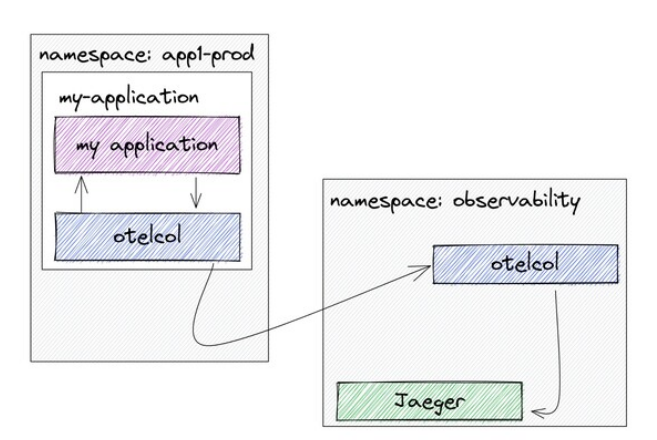
\includegraphics[scale=0.8]{gambar/sidecar-pattern}
        \caption{Deployment Opentelemetry Collector dengan sidecar.}
        \label{otel-collector-sidecar}
    \end{figure}
    
  \item Deployment menggunakan DaemonSet
  
  Berbeda dengan sidecar, DaemonSet menjalankan Opentelemetry Collector pada setiap node. Cara kerja dari pattern ini adalah setiap pod yang berada pada satu node akan mengirimkan data telemetri menuju OpenTelemetry Collector pada node tersebut yang kemudian akan mengirimkan data telemetri tersebut ke external collector seperti pada gambar 2.2

  \begin{figure}[H]
    \centering
      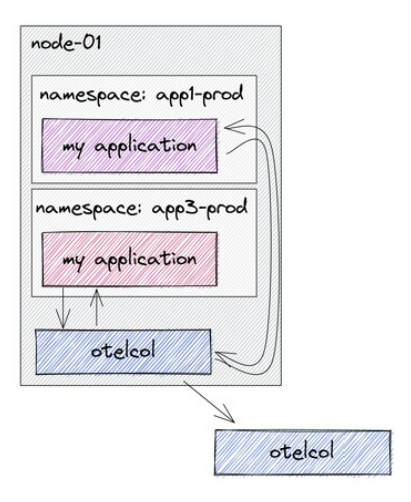
\includegraphics[scale=0.8]{gambar/daemonset-pattern}
      \caption{Deployment Opentelemetry Collector dengan daemonset.}
      \label{otel-collector-daemonset}
  \end{figure}

  \end{enumerate}

  Rolando Brondolin et al melakukan penelitian dengan mengembangkan sebuah pendekatan Black-box monitoring untuk mengukur runtime performa pada microservices. Penelitian ini menggunakan teknologi extended Berkeley Packet Filter (eBPF) yang digunakan untuk mengumpulkan data terkait performa aplikasi, penggunaan power, dan aktivitas network pada setiap docker container, kubernetes host dan physical host. eBPF merupakan sebuah teknologi yang memungkinkan penulis dapat membuat program yang berjalan di level kernel dengan aman, Dengan eBPF penulis dapat membuat sebuah program yang bertujuan untuk mengekstrak data metrics yang dibutuhkan untuk pengukuran performa aplikasi. Peneliti membuat dua eBPF program berbeda dengan tujuan masing-masing untuk mengumpulkan data performa dan data network. Kedua program tersebut bereaksi pada Linux tracepoint dan Kprobe yang khusus pada data yang ingin dikumpulkan. Ketika eBPF VM menerima event dari linux kernel, event tersebut akan dikirimkan menuju program eBPF yang telah dibuat sesuai dengan jenis event kemudian hasil dari program tersebut akan dikirim dan disimpan pada hash map yang dapat diakses oleh user-space agen. kemudian, user-space agen akan mengirimkan data yang telah dikumpulkan menuju remote backend.

\section{Landasan Teori}
  \subsection{Microservices}
  Microservices merupakan sebuah aristektur perangkat lunak yang terdiri dari banyak servis yang independen. Setiap servis mengenkapsulasi fungsi sebuah proses tertentu dan saling berkomunikasi melalui jaringan\cite{BuildingMicroservices}. Sebagai contoh sebuah aplikasi toko online yang terdiri dari beberapa servis yaitu inventory, account, dan shipping seperti pada gambar 2.1. 
  
  \begin{figure}[H]
    \centering
      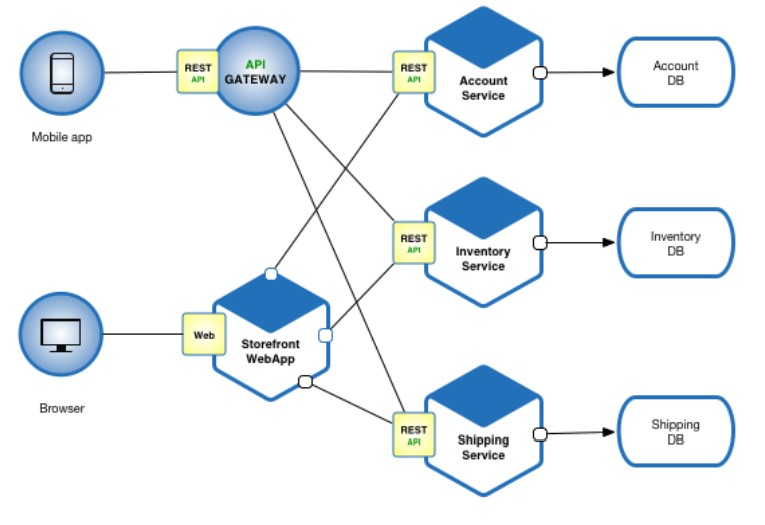
\includegraphics[scale=0.8]{gambar/microservices_architecture}
      \caption{Arsitektur microservices toko online.}
      \label{microservices}
  \end{figure}

  \subsection{Docker}
  Docker merupakan sebuah teknologi sumber terbuka yang berjalan di windows atau linux yang membantu dalam membuat, mengatur, dan melakukan orkestrasi kontainer. Kontainer merupakan sebuah paket ringan yang berisi kode perangkat lunak, environment serta dependensi lainnya. Kontainer memungkinkan sebuah aplikasi untuk berjalan di lingkungan yang terisolasi pada sebuah host seperti pada gambar 2.2.

  \begin{figure}[H]
    \centering
      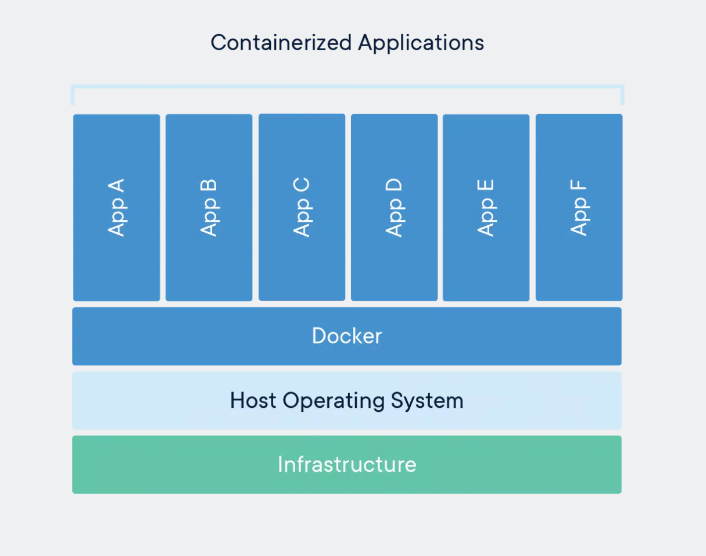
\includegraphics[scale=0.5]{gambar/docker-container}
      \caption{Kontainer yang berjalan pada sebuah host.}
      \label{containerized}
  \end{figure}

  \subsection{Kubernetes}
  Kubernetes merupakan sebuah platform sumber terbuka yang merupakan bagian dari Cloud Native Computing Foundation (CNCF). Kubernetes digunakan untuk melakukan manajemen container secara otomatis. Kubernetes memiliki kemampuan diantaranya load balancing, manajemen storage, otomasi rollouts dan rollback, pembatasan resource container, self-healing, dan manajemen konfigurasi\cite{Kubernetes}. 

  Sebuah kubernetes cluster terdiri dari beberapa node. Sebuah node dapat merupakan sebuah linux host yang berjalan baik pada mesin fisik atau virtual. Terdapat dua jenis node pada kubernetes yaitu control plane node dan worker node\cite{kubernetesNigelPoulton}. Sebuah control plane node beperan untuk mengatur dan mengontrol worker node sedangkan worker node berperan untuk menjalankan aplikasi yang berjalan pada sebuah kontainer sperti pada gambar.

  \begin{figure}[H]
    \centering
      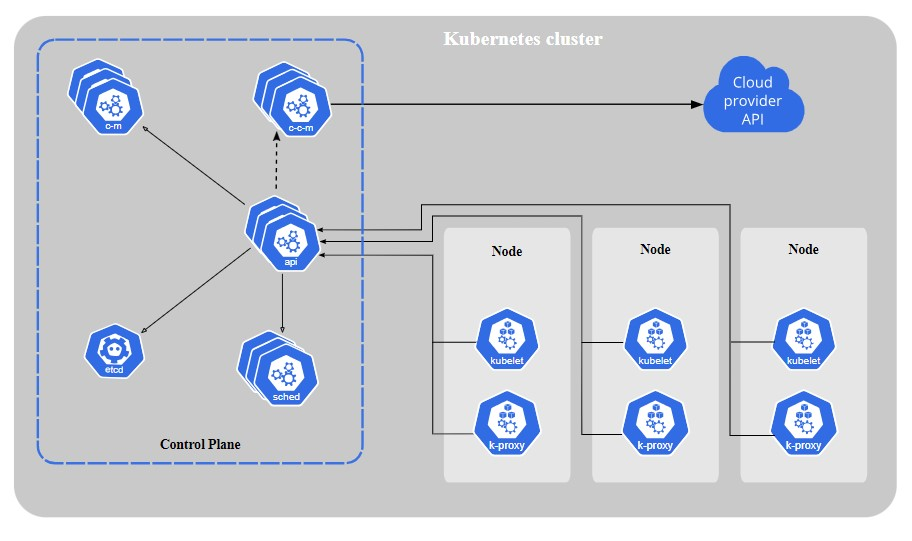
\includegraphics[scale=0.7]{gambar/kubernetes-component}
      \caption{Komponen-komponen pada kubernetes cluster.}
      \label{kubernetes-component}
  \end{figure}

  \subsection{Minikube}
  Minikube merupakan sebuah tool yang digunakan untuk menjalankan sebuah kubernetes cluster pada sebuah host lokal yang tersedia untuk Linux, macOS, dan Windows. Minikube bekerja dengan cara membuat sebuah virtual machine yang berisi sebuah single-node kubernetes cluster. Minikube dapat digunakan untuk melakukan eksperimen pada kubernetes atau untuk melakukan development aplikasi yang akan di deploy pada sebuah cluster kubernetes\cite{Minikube}.

  \subsection{Distributed Tracing}
  Tracing merupakan suatu metode untuk mengetahui serangkaian kejadian atau event yang terjadi pada sebuah request aplikasi. Sebuah tracing dikatakan distributed apabila dalam request tersebut melibatkan atau melewati beberapa proses atau mesin atau jaringan yang berbeda. Sebuah request digambarkan sebagai trace yang terdiri dari beberapa span, span tersebut merupakan unit terkecil kejadian yang terjadi pada sebuah trace. Gambar sebuah trace dapat dilihat pada gambar 2.4.
  
  \begin{figure}[H]
    \centering
      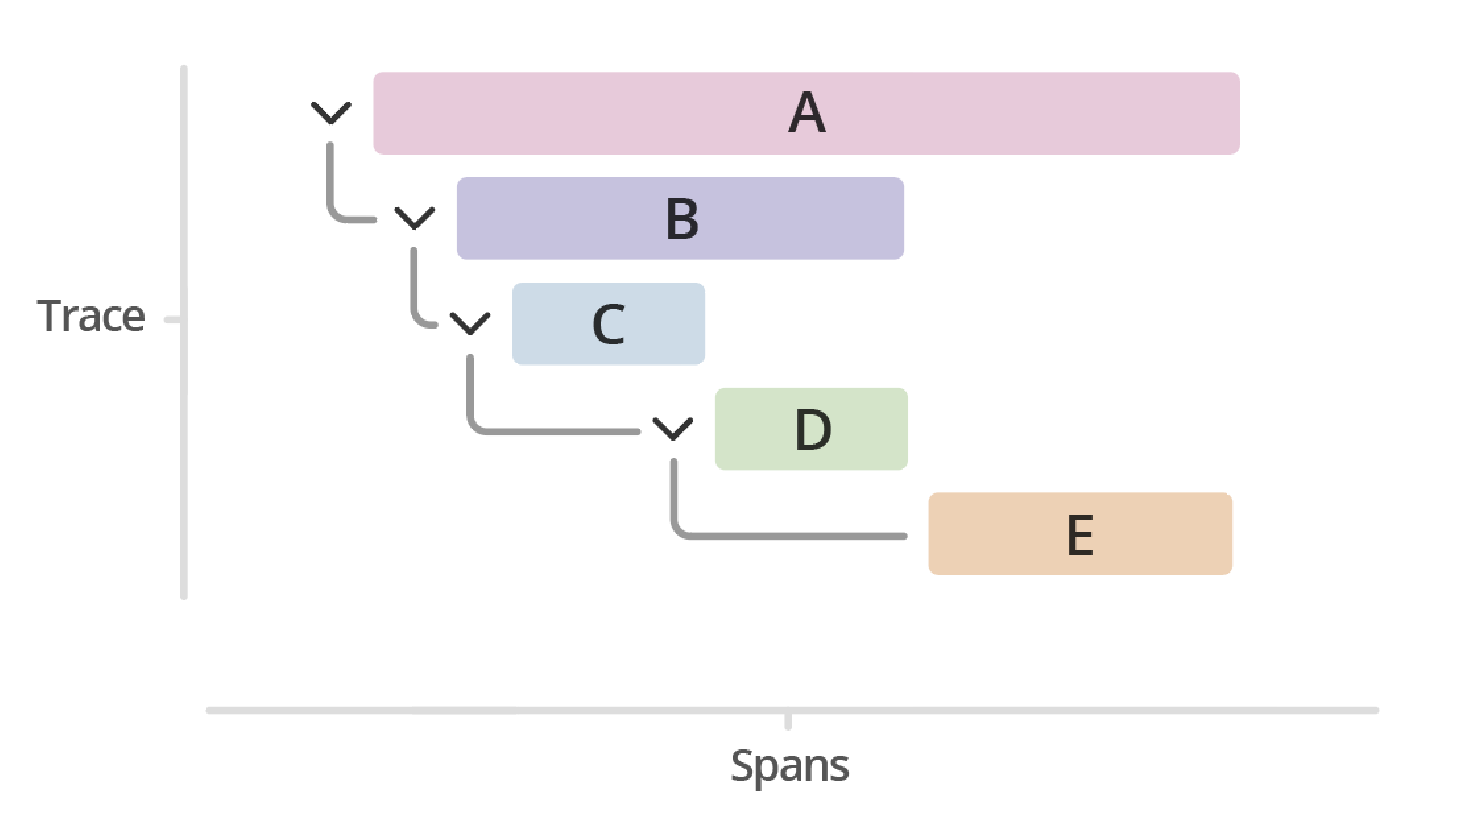
\includegraphics[scale=0.6]{gambar/traces-spans}
      \caption{Trace.}
      \label{Trace}
  \end{figure}

  Distributed tracing bekerja dengan cara menginstrumentasi aplikasi sehingga ketika sebuah request masuk aplikasi akan membuat sebuah traceID kemudian traceID tersebut akan dikirimkan ke setiap proses yang dilalui oleh request tersebut. Setiap proses akan membentuk sebuah span dengan spanID. Span akan menyimpan informasi seperti waktu mulai dan selesai, durasi, dan metadata terkait. Kemudian, trace dan span yang telah dibuat akan digabungkan sesuai urutannya oleh sebuah sistem atau platform distributed tracing.

  \subsection{OpenTelemetry}
  Opentelemetry merupakan observability framework yang bersifat sumber terbuka dan merupakan projek dari CNCF. Opentelemetry menyediakan standar, tools, APIs, dan SDKs yang dapat digunakan untuk instrumentasi, menghasilkan, mengumpulkan, dan mengeskport data telemetri (metrics, logs, traces) untuk membantu dalam analisis performance pada aplikasi. Opentelemetry besifat vendor-agnostic yang berarti dapat digunakan di bahasa dan teknologi banyak teknologi\cite{WhatIsOpentelemetry}.

  Opentelemetry terdiri dari beberapa komponen, yaitu

  \begin{enumerate}
    \item API and SDK\\
    Opentelemetry sudah menyediakan API (application programming interface) dan SDK (Software Development Kit) untuk berbagai macam bahasa pemrograman sehingga dapat membantu untuk melakukan instrumentasi pada aplikasi dengan berbagai bahasa untuk menghasilkan metrics dan tracing telemetri.
    \item OpenTelemetry Collector\\
    Opentelemetry collector merupakan sebuah implementasi yang bersifat vendor-agnostic untuk melakukan penerimaan, pemrosesan, dan mengirimkan data telemetri. dengan opentelemetry collector data telemetri dapat dikirimkan ke berbagai backend tools seperti Jaeger, Prometheus, Zipkin, dan lain-lain\cite{OtelCollector}. Arsitektur dari opentelemetry collector dapat dilihat pada gambar 2.5.

      \begin{figure}[H]
        \centering
          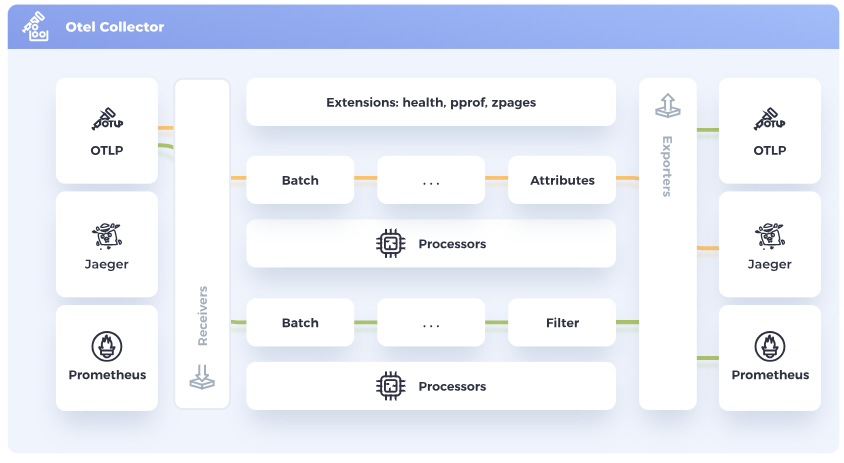
\includegraphics[scale=0.7]{gambar/otel-collector}
          \caption{Arsitektur Opentelemetry collector.}
          \label{Arsitektur Opentelemetry collector.}
      \end{figure}
      
    Gambar .... merupakan contoh data telemetri traces dengan standar Opentelemetry.

    \begin{figure}[H]
      \centering
        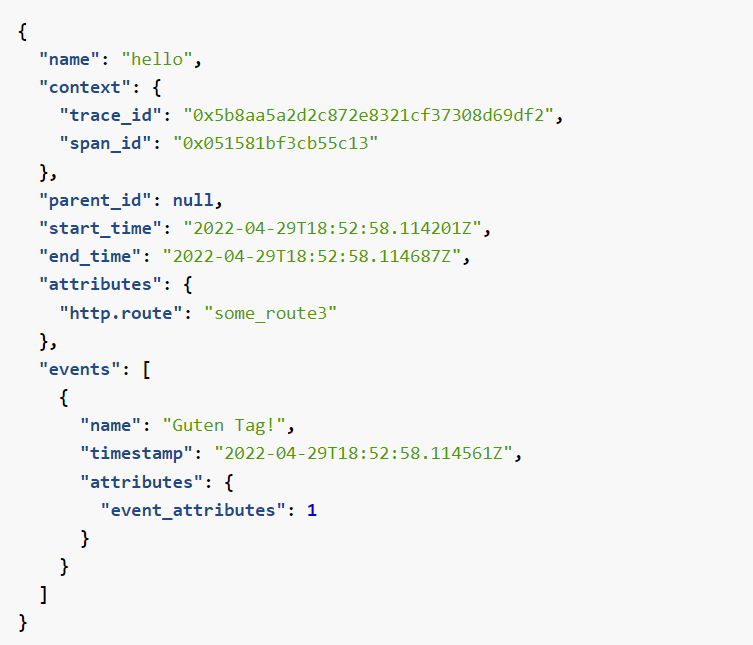
\includegraphics[scale=0.8]{gambar/otel-data-traces}
        \caption{OpenTelemetry data trace.}
        \label{Otel data trace.}
    \end{figure}

    \item OpenTelemetry Protocol\\
    OTLP merupakan protokol untuk mentransmisikan traces, metrics, dan logs telemetri. OTLP membantu Opentelemetry untuk mengirimkan data 13
    ke banyak backend tools. OTLP mengatur bagaimana encoding, transport, dan mekanisme pengiriman data.
  \end{enumerate}
  Bagaimana Opentelemetry bekerja dapat dilihat pada gambar Sebuah aplikasi akan menggunakan API dan SDK Opentelemetry untuk menginstrumentasi data telemetri kemudian data tersebut di proses sebelum di export/kirim menuju collector dan dari collector akan diexport menuju backend tools.

  \begin{figure}[H]
    \centering
      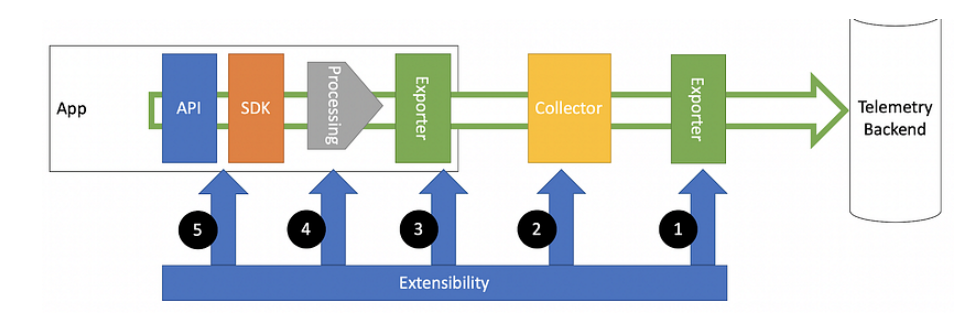
\includegraphics[scale=0.7]{gambar/otel-working}
      \caption{Alur kerja Opentelemetry}
      \label{Alur kerja Opentelemetry.}
  \end{figure}

  \subsection{REST API}
  Application Programming Interface atau API merupakan sekumpulan kode atau aturan yang mengizinkan dua aplikasi saling berkomunikasi. Salah satu jenis API ada REST API. REST (Representational State Transfer) API merupakan arsitektur API dimana komunikasi yang terjadi antar dua aplikasi bersifat stateless dan menggunakan protokol HTTP atau HTTPS. REST API menggunakan HTTP method seperti GET, POST, PUT, dan DELETE dan menggunakan JSON sebagai format penerimaan atau pengiriman data.

  \begin{figure}[H]
    \centering
      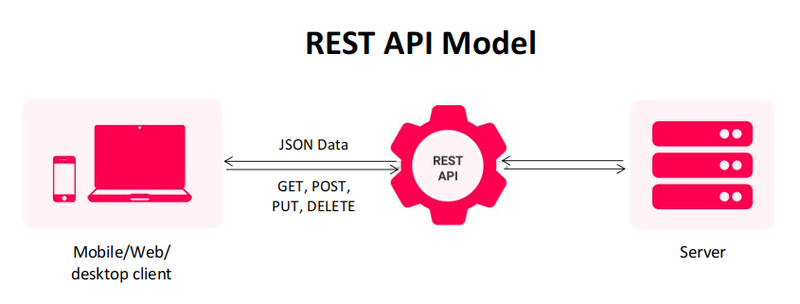
\includegraphics[scale=0.5]{gambar/rest-api}
      \caption{Alur kerja REST API.}
      \label{Alur kerja REST API.}
  \end{figure}

  Gambar 2.7 merupakan alur kerja dari sebuah REST API dimana sebuah klien melakukan request dengan method GET/POST/PUT/DELETE kemudian request tersebut akan diterima oleh server dan server akan mengirimkan response sesuai dengan request yang diterima dalam bentuk JSON seperti pada gambar .

  \begin{figure}[H]
    \centering
      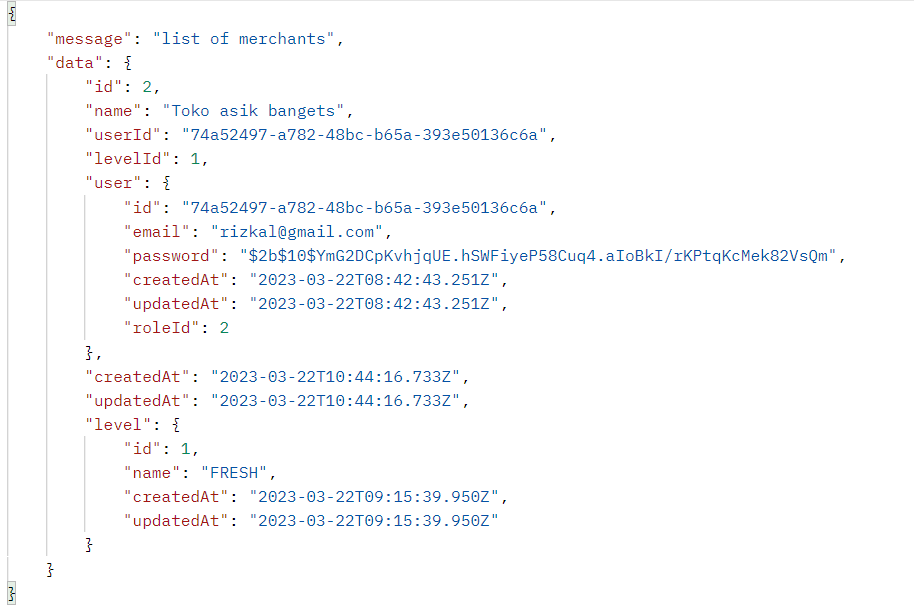
\includegraphics[scale=0.7]{gambar/json-example}
      \caption{Format data JSON.}
      \label{Format data JSON.}
  \end{figure}
  
  \subsection{Load Testing}
  Load testing merupakan salah satu jenis pengujian pada aplikasi perangkat lunak. Load testing menguji perangkat lunak dengan memberikan beban yang biasanya berupa request ke aplikasi untuk melihat apakah aplikasi tersebut mampu mengatasi beban tersebut dengan baik. Ada banyak tools sumber terbuka untuk melakukan load testing seperti k6, JMeter, Locust, dan lain-lain.

%!TEX root = ./template-skripsi.tex
%-------------------------------------------------------------------------------
%                            BAB III
%               		METODOLOGI PENELITIAN
%-------------------------------------------------------------------------------

\chapter{METODOLOGI PENELITIAN}

\section{Alat dan Bahan}
	Alat dan bahan yang digunakan pada penelitian ini terbagi atas perangkat keras dan perangkat lunak yang akan dijelaskan seperti berikut.

	\subsection{Perangkat Keras}
		Pro omnium incorrupte ea. Elitr eirmod ei qui, ex partem causae disputationi nec. Amet dicant no vis, eum modo omnes quaeque ad, antiopam evertitur reprehendunt pro ut. Nulla inermis est ne. Choro insolens mel ne, eos labitur nusquam eu, nec deserunt reformidans ut. His etiam copiosae principes te, sit brute atqui definiebas id.

		\vspace{-0.5cm}

		\begin{enumerate}[a.]
		\begin{singlespace}
		\itemsep0em
			\item Kit pancar-rima IQRF TR-53B (3 unit),
			\item Kit pengunduh program CK-USB-04 (1 unit),
			\item Kit pengembangan DK-EVAL-03 (2 unit),
			\item Kit pengembangan CK-EVAL-04 (1 unit),
			\item \emph{XBee 802.15.4 Radios (Series 1)} (3 unit),
			\item \emph{XBee Explorer USB Board} (1 unit),
			\item \emph{2 channel Relay Shield For Arduino (With XBee/BTBee interface)} (2 unit),
			\item Arduino Uno (2 unit),
			\item TP-LINK MR3020 (1 unit),
			\item Kabel USB ke Serial Prolific (1 unit).
		\end{singlespace}
		\end{enumerate}

	\subsection{Perangkat Lunak}
		Pro omnium incorrupte ea. Elitr eirmod ei qui, ex partem causae disputationi nec. Amet dicant no vis, eum modo omnes quaeque ad, antiopam evertitur reprehendunt pro ut. Nulla inermis est ne. Choro insolens mel ne, eos labitur nusquam eu, nec deserunt reformidans ut. His etiam copiosae principes te, sit brute atqui definiebas id.

		\vspace{-0.5cm}

		\begin{enumerate}[a.]
		\begin{singlespace}
		\itemsep0em
			\item Arduino for Mac OS X,
			\item CoolTerm,
			\item Driver FTDI for Mac OS X,
			\item PHP, MySQL, dan uHTTPd,
			\item Python dan pustaka PySerial,
			\item IQRF IDE v 2.08 for TR-53B,
			\item SSHFS,
			\item Sublime Text 3.
		\end{singlespace}
		\end{enumerate}

\section{Alur Penelitian}
	Consul graeco signiferumque qui id, usu eu summo dicunt voluptatum, nec ne simul perpetua posidonium. Eos ea saepe prodesset signiferumque. No dolore possit est. Mei no justo intellegebat definitiones, vis ferri lorem eripuit ad. Solum tritani scribentur duo ei, his an adipisci intellegat.

\section{Tahapan Pelaksanaan}
	Consul graeco signiferumque qui id, usu eu summo dicunt voluptatum, nec ne simul perpetua posidonium. Eos ea saepe prodesset signiferumque. No dolore possit est. Mei no justo intellegebat definitiones, vis ferri lorem eripuit ad. Solum tritani scribentur duo ei, his an adipisci intellegat.

\section{Jadwal Kegiatan}
	Quo no atqui omnesque intellegat, ne nominavi argumentum quo. Eum ei purto oporteat dissentiet, soleat utamur an sit. Et assum dicam interpretaris quo. Cetero alterum ea vel, no possit alterum utroque nec. His fuisset quaestio ad. Has eu tritani incorrupte consequuntur, esse aliquip nec ne \ref{jadwal}.

	% Please remember to add \use{multirow} to your document preamble in order to suppor multirow cells
		\begin{table}[H]
		\centering
		\caption{Jadwal Penelitian.}
		\label{jadwal}
		\begin{tabular}{|c|l|l|l|l|l|l|l|}
		\hline
		\multirow{2}{*}{No} & \multirow{2}{*}{Keterangan} & \multicolumn{6}{c|}{Bulan}                                                                                                                          \\ \cline{3-8} 
		                    &                             & 1 & 2 & 3 & 4 & 5 & 6 \\ \hline
		1                   & Studi literatur                                  &\cellcolor{gray} &\cellcolor{gray}&                        &                        &                        &                         \\ \hline
		2                   & Desain                                           &                        &\cellcolor{gray}&\cellcolor{gray}&                        &                        &                         \\ \hline
		3                   & Pembelian bahan                                  &                        &                        &\cellcolor{gray}&                        &                        &                         \\ \hline
		4                   & Pembuatan prototipe                              &                        &                        &\cellcolor{gray}&\cellcolor{gray}&\cellcolor{gray}&                         \\ \hline
		5                   & Uji coba dan perbaikan                           &                        &                        &                        &\cellcolor{gray}&\cellcolor{gray}&                         \\ \hline
		6                   & Penulisan skripsi                                &                        &                        &                        &                        &                        &\cellcolor{gray}\\ \hline
		\end{tabular}
		\end{table}
	
% Baris ini digunakan untuk membantu dalam melakukan sitasi
% Karena diapit dengan comment, maka baris ini akan diabaikan
% oleh compiler LaTeX.
\begin{comment}
\bibliography{daftar-pustaka}
\end{comment}


%!TEX root = ./template-skripsi.tex
%-------------------------------------------------------------------------------
%                            BAB IV
%               		HASIL DAN PEMBAHASAN
%-------------------------------------------------------------------------------

\chapter{HASIL DAN PEMBAHASAN}
	\section{Subbab 1}
		Habeo perfecto in sea. Ea deleniti gloriatur pri, paulo mediocrem incorrupte sea ei. Ad mollis scripta per. Incorrupte sadipscing ne mel. Mel ex nonumy malorum epicurei.

		Ne per tota mollis suscipit. Ullum labitur vim ut, ea dicit eleifend dissentias sit. Duis praesent expetenda ne sed. Sit et labitur albucius elaboraret. Ceteros efficiantur mei ad. Hendrerit vulputate democritum est at, quem veniam ne has, mea te malis ignota volumus.

		Eros reprimique vim no. Alii legendos volutpat in sed, sit enim nemore labores no. No odio decore causae has. Vim te falli libris neglegentur, eam in tempor delectus dignissim, nam hinc dictas an.
	
	\section{Subbab 2}		
		Habeo perfecto in sea. Ea deleniti gloriatur pri, paulo mediocrem incorrupte sea ei. Ad mollis scripta per. Incorrupte sadipscing ne mel. Mel ex nonumy malorum epicurei.

		\subsection{Subsubbab 2 1}
			Ne per tota mollis suscipit. Ullum labitur vim ut, ea dicit eleifend dissentias sit. Duis praesent expetenda ne sed. Sit et labitur albucius elaboraret. Ceteros efficiantur mei ad. Hendrerit vulputate democritum est at, quem veniam ne has, mea te malis ignota volumus.
			
			\begingroup
			    \fontsize{10pt}{12pt}\selectfont
			    \begin{verbatim}
					config mount
				        option target        /mnt
				        option device        /dev/sda1
				        option fstype        ext3
				        option options       rw,sync
				        option enabled       1
				        option enabled_fsck  0
				        option is_rootfs     1
			    \end{verbatim}  
			\endgroup

			\begingroup
			    \fontsize{10pt}{12pt}\selectfont
			    \begin{verbatim}
					# opkg update
					# opkg install python pyserial
			    \end{verbatim}  
			\endgroup			

		\subsection{Subsubbab 2 2}
			Consul graeco signiferumque qui id, usu eu summo dicunt voluptatum, nec ne simul perpetua posidonium. Eos ea saepe prodesset signiferumque. No dolore possit est. Mei no justo intellegebat definitiones, vis ferri lorem eripuit ad. Solum tritani scribentur duo ei, his an adipisci intellegat.

	\section{Subab 3}
		Consul graeco signiferumque qui id, usu eu summo dicunt voluptatum, nec ne simul perpetua posidonium. Eos ea saepe prodesset signiferumque. No dolore possit est. Mei no justo intellegebat definitiones, vis ferri lorem eripuit ad. Solum tritani scribentur duo ei, his an adipisci intellegat.
			
			
% Baris ini digunakan untuk membantu dalam melakukan sitasi.
% Karena diapit dengan comment, maka baris ini akan diabaikan
% oleh compiler LaTeX.
\begin{comment}
\bibliography{daftar-pustaka}
\end{comment}

%!TEX root = ./template-skripsi.tex
%-------------------------------------------------------------------------------
%                            	BAB V
%               		KESIMPULAN DAN SARAN
%-------------------------------------------------------------------------------

\chapter{KESIMPULAN DAN SARAN}

\section{Kesimpulan}
	Berdasarkan hasil analisis dan pengujian fungsional aplikasi ini, didapat kesimpulan sebagai berikut:

	\begin{enumerate}
		\item Lorem ipsum is a pseudo-Latin text used in web design, typography, layout, and printing in place of English to emphasise design elements over content. 
		
		\item It's also called placeholder (or filler) text. It's a convenient tool for mock-ups. 
		
		\item It helps to outline the visual elements of a document or presentation, eg typography, font, or layout. Lorem ipsum is mostly a part of a Latin text by the classical author and philospher Cicero.

		\item Its words and letters have been changed by addition or removal, so to deliberately render its content nonsensical; it's not genuine, correct, or comprehensible Latin anymore. 
	\end{enumerate}


\section{Saran}
	\begin{enumerate}
		\item Lorem ipsum is a pseudo-Latin text used in web design, typography, layout, and printing in place of English to emphasise design elements over content. 
		
		\item It's also called placeholder (or filler) text. It's a convenient tool for mock-ups. 
		
		\item It helps to outline the visual elements of a document or presentation, eg typography, font, or layout. Lorem ipsum is mostly a part of a Latin text by the classical author and philospher Cicero.

		\item Its words and letters have been changed by addition or removal, so to deliberately render its content nonsensical; it's not genuine, correct, or comprehensible Latin anymore. 
	\end{enumerate}

	
% Baris ini digunakan untuk membantu dalam melakukan sitasi
% Karena diapit dengan comment, maka baris ini akan diabaikan
% oleh compiler LaTeX.
\begin{comment}
\bibliography{daftar-pustaka}
\end{comment}


%-----------------------------------------------------------------
%Disini akhir masukan Bab
%-----------------------------------------------------------------


%-----------------------------------------------------------------
% Disini awal masukan untuk Daftar Pustaka
% - Daftar pustaka diambil dari file .bib yang ada pada folder ini
%   juga.
% - Untuk memudahkan dalam memanajemen dan menggenerate file .bib
%   gunakan reference manager seperti Mendeley, Zotero, EndNote,
%   dll.
%-----------------------------------------------------------------
\bibliography{IEEEabrv,daftar-pustaka}
\addcontentsline{toc}{chapter}{DAFTAR PUSTAKA}
%-----------------------------------------------------------------
%Disini akhir masukan Daftar Pustaka
%-----------------------------------------------------------------

\end{document}